\documentclass[
    12pt, % Schriftgröße
    DIV10,
    ngerman, % für Umlaute, Silbentrennung etc.
    a4paper, % Papierformat
    oneside, % einseitiges Dokument
    titlepage, % es wird eine Titelseite verwendet
    parskip=half, % Abstand zwischen Absätzen (halbe Zeile)
    headings=normal, % Größe der Überschriften verkleinern
    listof=totoc, % Verzeichnisse im Inhaltsverzeichnis aufführen
    bibliography=totoc, % Literaturverzeichnis im Inhaltsverzeichnis aufführen
    index=totoc, % Index im Inhaltsverzeichnis aufführen
    captions=tableheading, % Beschriftung von Tabellen unterhalb ausgeben
    final % Status des Dokuments (final/draft)
]{scrartcl}

% Pakete

% Schrift ----------------------------------------------------------------------
\usepackage{lmodern} % bessere Fonts

% Paket für Kopfzeilen und Fußzeilen
\usepackage[
    automark, % Kapitelangaben in Kopfzeile automatisch erstellen
    headsepline, % Trennlinie unter Kopfzeile
    ilines % Trennlinie linksbündig ausrichten
]{scrpage2}

% Anpassung an Landessprache
\usepackage[ngerman]{babel}

% Umlaute ----------------------------------------------------------------------
%   Umlaute/Sonderzeichen wie äöüß direkt im Quelltext verwenden (CodePage).
%   Erlaubt automatische Trennung von Worten mit Umlauten.
% ------------------------------------------------------------------------------
\usepackage[utf8]{inputenc}
\usepackage[T1]{fontenc}
\usepackage{textcomp} % Euro-Zeichen etc.

\usepackage[babel,german=quotes]{csquotes}

% Bei Änderungen müssen die *.aux und *.bbl Dateien manuell gelöscht werden
% Sonst kommt es zu einem Fehler bei der Erstellung
%\usepackage[round, sort, comma, numbers]{natbib}
%\usepackage[round, numbers]{natbib}
%\bibliographystyle{abbrvdin}
%

\usepackage{scrhack}

\usepackage[citestyle=alphabetic,bibstyle=alphabetic,backend=biber]{biblatex}
\bibliography{Bibliographie}
\DefineBibliographyStrings{german}{
  bibliography = {Literaturverzeichnis},
}
\setlength\bibitemsep{8pt}

\usepackage{xpatch}
\xpretobibmacro{author}{\mkbibbold\bgroup}{}{}
\xapptobibmacro{author}{\egroup}{}{}
\xpretobibmacro{editor}{\mkbibbold\bgroup}{}{}
\xapptobibmacro{editor}{\egroup}{}{}
\xpretobibmacro{editor+others}{\mkbibbold\bgroup}{}{}
\xapptobibmacro{editor+others}{\egroup}{}{}
\xpretobibmacro{bbx:editor}{\mkbibbold\bgroup}{}{}
\xapptobibmacro{bbx:editor}{\egroup}{}{}

% Grafiken ---------------------------------------------------------------------
% Einbinden von JPG-Grafiken ermöglichen
\usepackage[dvips,final]{graphicx}
\graphicspath{{Bilder/}}

% Paket zur Verwendung zusätzlicher Positionsbefehle
\usepackage{float}

% Befehle aus AMSTeX für mathematische Symbole z. B. \boldsymbol \mathbb --------
\usepackage{amsmath,amsfonts}

% Einfache Definition der Zeilenabstände und Seitenränder etc. -----------------
\usepackage{setspace}
\usepackage{geometry}

% zum Umfließen von Bildern ----------------------------------------------------
\usepackage{floatflt}

% Farbdefinitionen
\usepackage{xcolor} 
\definecolor{hellgelb}{rgb}{1,1,0.9}
\definecolor{colKeys}{rgb}{0,0,1}
\definecolor{colIdentifier}{rgb}{0,0,0}
\definecolor{colComments}{rgb}{1,0,0}
\definecolor{colString}{rgb}{0,0.5,0}
\definecolor{whgreen}{RGB}{113,177,41}
\definecolor{dvBlue}{RGB}{0,85,160}

% URL verlinken, lange URLs umbrechen etc. -------------------------------------
\usepackage{url}

% PDF-Optionen -----------------------------------------------------------------
\usepackage[
    bookmarks,
    bookmarksopen=true,
    colorlinks=true,
% diese Farbdefinitionen zeichnen Links im PDF farblich aus
    linkcolor=dvBlue, % einfache interne Verkn�pfungen
    anchorcolor=black,% Ankertext
    citecolor=dvBlue, % Verweise auf Literaturverzeichniseintr�ge im Text
    filecolor=magenta, % Verkn�pfungen, die lokale Dateien �ffnen
    menucolor=dvBlue, % Acrobat-Men�punkte
    urlcolor=dvBlue, 
% diese Farbdefinitionen sollten für den Druck verwendet werden (alles schwarz)
%    linkcolor=black, % einfache interne Verkn�pfungen
%    anchorcolor=black, % Ankertext
%    citecolor=black, % Verweise auf Literaturverzeichniseintr�ge im Text
%    filecolor=black, % Verkn�pfungen, die lokale Dateien �ffnen
%    menucolor=black, % Acrobat-Men�punkte
%    urlcolor=black, 
    %backref, % Inkompatibel mit BibLateX
    plainpages=false, % zur korrekten Erstellung der Bookmarks
    pdfpagelabels, % zur korrekten Erstellung der Bookmarks
    hypertexnames=false, % zur korrekten Erstellung der Bookmarks
    linktocpage % Seitenzahlen anstatt Text im Inhaltsverzeichnis verlinken
]{hyperref}

% fortlaufendes Durchnummerieren der Fußnoten ----------------------------------
\usepackage{chngcntr}
%\counterwithout{footnote}{chapter}

% Formatierung von Listen ändern -----------------------------------------------
\usepackage{paralist} % itemize, enumerate

% bei der Definition eigener Befehle benötigt
\usepackage{ifthen} % Vielleicht nicht nötig

% definiert u.a. die Befehle \ und \listoftodos
\usepackage{todonotes}
\reversemarginpar

% sorgt dafür, dass Leerzeichen hinter parameterlosen Makros nicht als Makroendezeichen interpretiert werden
\usepackage{xspace}

\usepackage{tabularx} % Tabellenspalten mit variabler Breite
\usepackage{wrapfig}  % Schriftumflossene Bilder


% Seitenstil

% Zeilenabstand 1,5 Zeilen
\onehalfspacing

% Seitenränder
% bottom is 20 + X, weil Footer nicht berücksichtigt wird
\geometry{paper=a4paper,left=30mm,right=20mm,top=20mm, bottom=38mm, footskip=8mm}

% Kopf- und Fußzeilen ----------------------------------------------------------
% Kopf- und Fußzeile auch auf Kapitelanfangsseiten
%\renewcommand*{\chapterpagestyle}{scrheadings} 
% Schriftform der Kopfzeile
%\renewcommand{\headfont}{\normalfont}

% Kopfzeile
\ihead{\headmark} % links
\chead{}
\ohead{
\includegraphics[scale=0.04]{Bilder/Deckblatt/homebacon.png}} % rechts
\setlength{\headheight}{20mm} % Höhe der Kopfzeile
% Kopfzeile über den Text hinaus verbreitern
%\setheadwidth[0pt]{textwithmarginpar} 
\setheadsepline[text]{0.4pt} % Trennlinie unter Kopfzeile

% Fußzeile
%\ifoot{} % links
\cfoot{} % mitte
\ofoot{\pagemark} % rechts
%\setfootsepline[text]{0.4pt} % Trennlinie unter Kopfzeile



% Schusterjungen und Hurenkinder vermeiden
%\clubpenalty = 10000
%\widowpenalty = 10000 
%\displaywidowpenalty = 10000

% Verringert den Abstand über den Überschriften
%\renewcommand*{\chapterheadstartvskip}{\vspace*{-\topskip}}

% Irgendwas mit Silbentrennung in MonoSpace (texttt)
\newcommand{\origttfamily}{}% sollte noch nicht definiert sein!
\let\origttfamily=\ttfamily % alte Definition von \ttfamily sichern
\renewcommand{\ttfamily}{\origttfamily \hyphenchar\font=`\-}


% Eigene Befehle und typographische Auszeichnungen für diese

\newcommand{\bs}{$\backslash$}

% einige Befehle zum Zitieren --------------------------------------------------
\newcommand{\Zitat}[2][\
empty]{\ifthenelse{\equal{#1}{\empty}}{\citep{#2}}{\citep[#1]{#2}}}

% zum Ausgeben von Autoren
\newcommand{\AutorName}[1]{\textsc{#1}}
\newcommand{\Autor}[1]{\AutorName{\citeauthor{#1}}}

% Produktnamen
\newcommand{\produkt}[1]{\textbf{#1}}

\newcommand{\code}[1]{\texttt{#1}}

% zum Einbinden von Programmcode -----------------------------------------------
\usepackage{listings}
\usepackage{xcolor}
\usepackage{textcomp}
\lstset{
    float=hbp,
    basicstyle=\ttfamily\color{black}\small,
    identifierstyle=\color{colIdentifier},
    keywordstyle=\color{colKeys},
    stringstyle=\color{colString},
    commentstyle=\color{colComments},
    %columns=flexible,
    tabsize=2,
    frame=single,
    extendedchars=true,
    showspaces=false,
    showstringspaces=false,
    numbers=left,
    numberstyle=\ttfamily\small,
    numbersep=5pt,
    breaklines=true,
    backgroundcolor=\color{hellgelb},
    breakautoindent=true
}

\lstset{literate=
  {á}{{\'a}}1 {é}{{\'e}}1 {í}{{\'i}}1 {ó}{{\'o}}1 {ú}{{\'u}}1
  {Á}{{\'A}}1 {É}{{\'E}}1 {Í}{{\'I}}1 {Ó}{{\'O}}1 {Ú}{{\'U}}1
  {à}{{\`a}}1 {è}{{\'e}}1 {ì}{{\`i}}1 {ò}{{\`o}}1 {ù}{{\`u}}1
  {À}{{\`A}}1 {È}{{\'E}}1 {Ì}{{\`I}}1 {Ò}{{\`O}}1 {Ù}{{\`U}}1
  {ä}{{\"a}}1 {ë}{{\"e}}1 {ï}{{\"i}}1 {ö}{{\"o}}1 {ü}{{\"u}}1
  {Ä}{{\"A}}1 {Ë}{{\"E}}1 {Ï}{{\"I}}1 {Ö}{{\"O}}1 {Ü}{{\"U}}1
  {â}{{\^a}}1 {ê}{{\^e}}1 {î}{{\^i}}1 {ô}{{\^o}}1 {û}{{\^u}}1
  {Â}{{\^A}}1 {Ê}{{\^E}}1 {Î}{{\^I}}1 {Ô}{{\^O}}1 {Û}{{\^U}}1
  {œ}{{\oe}}1 {Œ}{{\OE}}1 {æ}{{\ae}}1 {Æ}{{\AE}}1 {ß}{{\ss}}1 {Δ}{{$\Delta$}}1
  {ç}{{\c c}}1 {Ç}{{\c C}}1 {ø}{{\o}}1 {å}{{\r a}}1 {Å}{{\r A}}1
  {€}{{\EUR}}1 {£}{{\pounds}}1
}

\usepackage{microtype}

\renewcommand*{\dictumwidth}{.41\textwidth}
\renewcommand*{\dictumrule}{}
\renewcommand*{\dictumauthorformat}[1]{--- #1}
\setkomafont{dictumauthor}{%
\scshape
}

\definecolor{bluekeywords}{rgb}{0,0,1}
\definecolor{greencomments}{rgb}{0,0.5,0}
\definecolor{redstrings}{rgb}{0.64,0.08,0.08}
\definecolor{xmlcomments}{rgb}{0.5,0.5,0.5}
\definecolor{types}{rgb}{0.17,0.57,0.68}

\lstdefinestyle{csharp}
{
    language=[Sharp]C,
    captionpos=b,
    %numbers=left, %Nummerierung
    %numberstyle=\tiny, % kleine Zeilennummern
    showspaces=false,
    showtabs=false,
    breaklines=true,
    showstringspaces=false,
    breakatwhitespace=true,
    escapeinside={(*@}{@*)},
    commentstyle=\color{greencomments},
    morekeywords={partial, var, value, get, set},
    keywordstyle=\color{bluekeywords},
    stringstyle=\color{redstrings},
    basicstyle=\ttfamily\small,
}

\lstdefinestyle{hive}
{
    language=SQL,
    captionpos=b,
    %numbers=left, %Nummerierung
    %numberstyle=\tiny, % kleine Zeilennummern
    showspaces=false,
    showtabs=false,
    breaklines=true,
    showstringspaces=false,
    breakatwhitespace=true,
    escapeinside={(*@}{@*)},
    commentstyle=\color{greencomments},
    morekeywords={bigint, double, decimal, char, string, row, format, lines, location, DELIMITED, FIELDS, TERMINATED, STORED, TEXTFILE,
    	OVERWRITE, DIRECTORY},
    keywordstyle=\color{bluekeywords},
    stringstyle=\color{redstrings},
    basicstyle=\ttfamily\small,
}

\lstdefinestyle{xml}
{
    language=XML,
    captionpos=b,
    %numbers=left, %Nummerierung
    %numberstyle=\tiny, % kleine Zeilennummern
    showspaces=false,
    showtabs=false,
    breaklines=true,
    showstringspaces=false,
    breakatwhitespace=true,
    escapeinside={(*@}{@*)},
    commentstyle=\color{greencomments},
    morekeywords={encoding},
    keywordstyle=\color{bluekeywords},
    stringstyle=\color{redstrings},
    basicstyle=\ttfamily\small,
}

\colorlet{punct}{red!60!black}
\definecolor{background}{HTML}{EEEEEE}
\definecolor{delim}{RGB}{20,105,176}
\colorlet{numb}{magenta!60!black}

\lstdefinelanguage{json}{
    basicstyle=\normalfont\ttfamily,
    numbers=left,
    numberstyle=\scriptsize,
    stepnumber=1,
    numbersep=8pt,
    showstringspaces=false,
    breaklines=true,
    frame=single,
    literate=
     *{0}{{{\color{numb}0}}}{1}
      {1}{{{\color{numb}1}}}{1}
      {2}{{{\color{numb}2}}}{1}
      {3}{{{\color{numb}3}}}{1}
      {4}{{{\color{numb}4}}}{1}
      {5}{{{\color{numb}5}}}{1}
      {6}{{{\color{numb}6}}}{1}
      {7}{{{\color{numb}7}}}{1}
      {8}{{{\color{numb}8}}}{1}
      {9}{{{\color{numb}9}}}{1}
      {:}{{{\color{punct}{:}}}}{1}
      {,}{{{\color{punct}{,}}}}{1}
      {\{}{{{\color{delim}{\{}}}}{1}
      {\}}{{{\color{delim}{\}}}}}{1}
      {[}{{{\color{delim}{[}}}}{1}
      {]}{{{\color{delim}{]}}}}{1},
}

%\usepackage{caption} 
%\captionsetup[table]{skip=100pt}
% Bindet die Literaturdaten ein!
\bibliography{Bibliographie}
\begin{document}

%Startstruktur
\setcounter{secnumdepth}{3}
\setcounter{tocdepth}{2}

\pagestyle{empty}
\thispagestyle{plain}
\begin{titlepage}

\begin{center}


\includegraphics[scale=0.7]{Deckblatt/WH_Logo.jpg}

\vspace{2cm}

\Huge{\textbf{Home Bacon}}\\[1.5ex]
\Large{\textbf{Projektdokumentation}}
\rule{\textwidth}{0.4pt}\\[3.0ex]

\large{\textbf{im Masterstudiengang Verteilte Systeme}}\\[3.0ex]

\normalsize
\begin{tabular}{ll}\\
	vorgelegt von: 
	& \quad Daniel Hardes,  Dennis Miller, \\[1.2ex]
	& \quad Fabian Paus, Christian Schlütter,\\[1.2ex]
	& \quad \\[1.2ex]
	Modul:  & \quad Mobile Computing (MOC) \\[1.2ex]
	Gutachter:  & \quad Prof. Dr. Martin Schulten \\[1.2ex]
	Abgabetermin:  & \quad \today\\[1.2ex]
\end{tabular}

\end{center}

\end{titlepage}


\tableofcontents
\setcounter{page}{1}

\pagestyle{scrheadings}

\newpage

\section{Projekt}

In dem Projekt "`Home Bacon"' wollen wir das Thema Lokalisierung via
Bluetooth-Beacons auf Smartwatches untersuchen und als Prototyp implementieren.

\subsection{Ergebnis}
Das Ergebnis vom Projekt sind 2 mobile Applikation, eine für ein Android Smartphone und eine für eine Android Wear Smartwatch. Diese beiden Apps werden Daten untereinander austauschen, jedoch keinen externen Server benötigen.

\subsection{Anwendungsfälle}
Wir möchten unsere Projektidee und unsere Anforderungen in Form von Userstories und Anwendungsfällen konkretisieren. Dazu haben wir uns den fiktiven Anwender Anton ausgedacht, der sehr vergesslich aber experimentierfreudig ist. Als Technik-affiner Mensch, hat Anton natürlich eine moderne Smartwatch und ein Smartphone. Aufgrund seiner Vergesslichkeit wünscht sich Anton verlegte Gegenstände wie Schlüsselbunde leichter wiederfinden zu können. Außerdem möchte er beim Verlassen des Hauses an seine Einkaufsliste erinnert werden.

Nachfolgend werden Antons Wünsche detaillierter ausgeführt.

\subsubsection{Positionierung}
\begin{figure}[H]
\centering
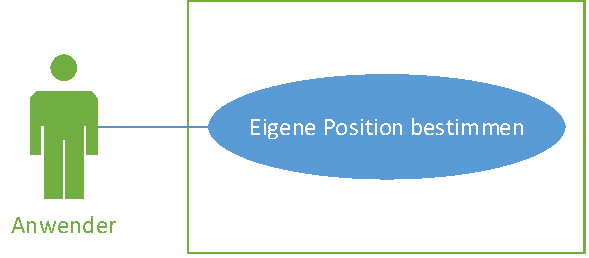
\includegraphics[width=0.7\linewidth]{Bilder/UseCase-Position}
\caption{Anwendungsfalldiagramm Positionierung}
\label{fig:UseCase-Position}
\end{figure}

\newpage
Als Anwender Anton möchte ich meine eigene Position in meinem Haus bestimmen können, um zu wissen in welchem Raum ich mich befindet. 

Akzeptanzkriterien:
\begin{itemize}
\item Die Smartwatch zeigt die aktuelle Position als Raumbezeichnung an.
\end{itemize}

Als Anwender Anton möchte ich wissen, wo sich ein verlegter Gegenstand befindet, um diesen leichter wiederfinden zu können.

Akzeptanzkriterien:
\begin{itemize}
\item Auf der Smartwatch kann aus allen getrackten Gegenstände der gesuchte ausgewählt werden.
\item Zu dem ausgewählten Gegenstand wird die zuletzt wahrgenommene Position angezeigt.
\item Die Smartwatch gibt Feedback abhängig von der Nähe zum Gegenstand.
\end{itemize}

\subsubsection{Notizen}
\begin{figure}[H]
\centering
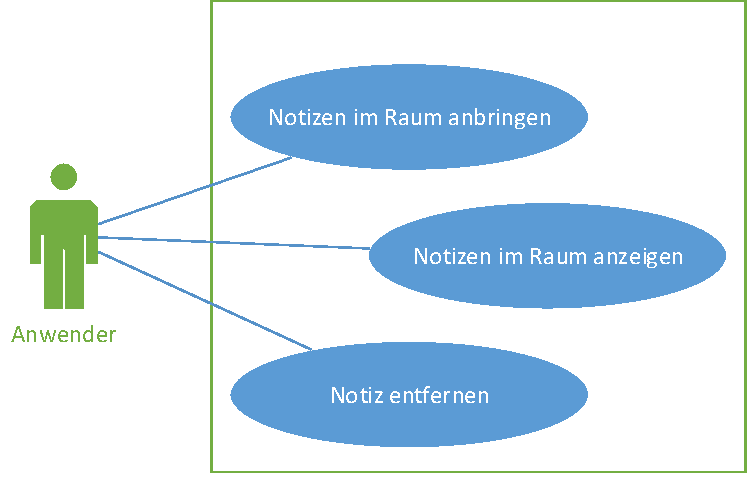
\includegraphics[width=0.7\linewidth]{Bilder/UseCase-Notizen}
\caption{Anwendungsfalldiagramm Notizen}
\label{fig:UseCase-Notizen}
\end{figure}

Als Anwender Anton möchte ich Notizen im Raum anbringen können, um diese zur späteren Ansicht zu hinterlassen.

Akzeptanzkriterien:
\begin{itemize}
\item Notizen können über das Smartphone im aktuellen Raum hinterlassen werden.
\end{itemize}

Als Anwender Anton möchte ich Notizen im Raum angezeigt bekommen, um hinterlassene Notizen zu lesen.

Akzeptanzkriterien:
\begin{itemize}
\item Auf der Smartwatch wird zuerst die aktuellste Notiz angezeigt.
\item Mithilfe der horizontalen Wischgeste sind ältere Notizen abrufbar.
\end{itemize}

Als Anwender Anton möchte ich Notizen löschen können, um alte Notizen zu entfernen.

Akzeptanzkriterien:
\begin{itemize}
\item Auf der Smartwatch kann mithilfe der vertikalen Wischgeste die angezeigte Notiz gelöscht werden.
\item Bevor die Notiz endgültig gelöscht wird, muss das Löschen bestätigt werden.
\end{itemize}

\subsubsection{Ereignisse}
\begin{figure}[H]
\centering
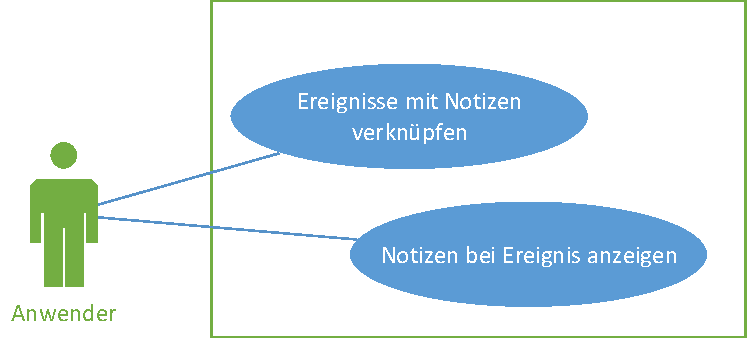
\includegraphics[width=0.7\linewidth]{Bilder/UseCase-Ereignisse}
\caption{Anwendungsfalldiagramm Ereignisse}
\label{fig:UseCase-Ereignisse}
\end{figure}

Als Anwender Anton möchte ich Ereignisse mit Notizen verknüpfen, um beim Verlassen bzw. Betreten eines Raumes die Notizen angezeigt zu bekommen.

Akzeptanzkriterien:
\begin{itemize}
\item Auf dem Smartphone können Notizen mit den zwei Ereignissen (Betreten bzw. Verlassen) verknüpft werden.
\end{itemize}

\newpage
Als Anwender Anton möchte ich die Notizen angezeigt bekommen, wenn ich einen Raum betrete bzw. verlasse, um an die Notiz erinnert zu werden.

Akzeptanzkriterien:
\begin{itemize}
\item Mittels der Smartwatch erhält Anton Feedback, wenn ein Ereignis mit verknüpften Notizen eintritt.
\item Auf der Smartwatch werden dann diese verknüpften Notizen angezeigt.
\end{itemize}


\subsection{Projektplan}

In folgendem Diagramm haben wir unsere Zeitplanung für das Projekt aufgezeichnet.

\begin{figure}[tbh]
\centering
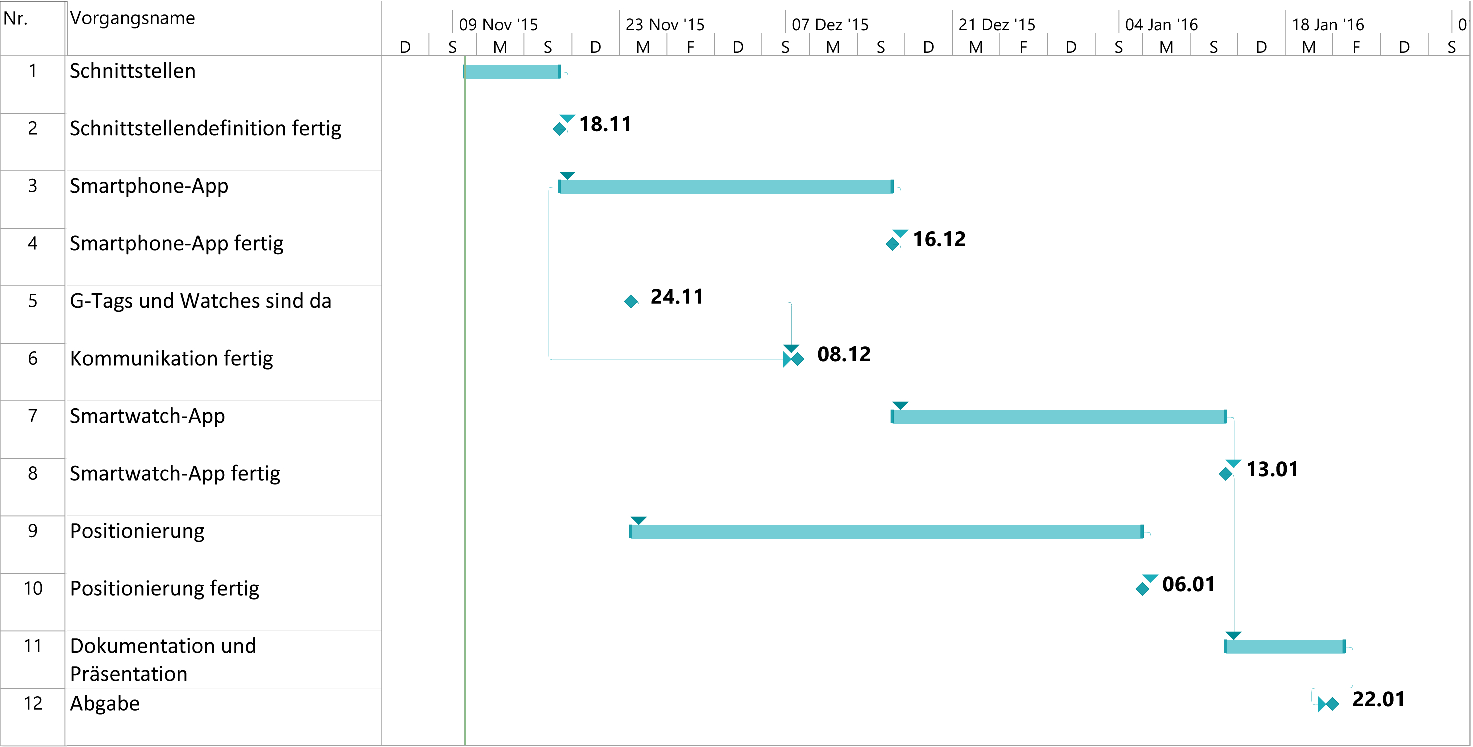
\includegraphics[width=1.0\linewidth]{Bilder/Projektplan}
\caption{Zeitplan mit Meilensteinen}
\label{fig:Zeitplan-1}
\end{figure}

\subsubsection{Projektphasen}
\begin{description}
	\item[Schnittstellen:] Definition der Schnittstellen zur Positionsbestimmung und zur Kommunikation zwischen
	Smartphone und Smartwatch. Dadurch können gewisse Teile unabhängig voneinander entwickelt werden.
	\item[Smartphone-App] Entwicklung der Smartphone-App zur Hinterlegung von Notizen in Räumen und bei Ereignissen.
	\item[Smartwatch-App] Entwicklung der Smartwatch-App zur Anzeige von Notizen in Räumen und bei Ereignissen sowie
	dem Wiederfinden von Gegenständen.
	\item[Positionierung] Bestimmung der Position der Smartwatch anhand der Bluetooth-Signale der stationären Tags.
	\item[Dokumentation und Präsentation] Erstellung der Dokumentation und Vorbereitung der Präsentation.
\end{description}

\subsubsection{Meilensteine}
\begin{description}
	\item[Schnittstellendefinition] Schnittstellen sind festegelegt.
	\item[G-Tags und Watches sind da] Geschätzter Termin für das Eintreffen der bestellten Ware.
	\item[Smartphone $\rightarrow$ Smartwatch] Kommunikation von der Smartphone-App mit der Smartwatch ist implementiert.
	\item[Smartphone-App] Die Smartphone-App ist fertig (ggf. Mock-Implementierungen für die Schnittstellen)
	\item[Positionierung] Die Positionierung auf der Smartwatch ist fertig.
	\item[Smartwatch-App] Die Smartwatch-App ist fertig.
	\item[Abgabe] Die Dokumentation wurde abgegeben.
\end{description}


%\section{Einordnung in Mobile Computing}
%Hier soll die Anwendung in gemäß den Inhalten der Vorlesung eingeordnet werden.
%\\- Arten der Mobilität
%
%Abstraktionen
%\\- Modell: Lokation und Kontext beschreiben
%\\- Algorithmen: Vorwiegend zur Lokation und ggf. für Ausführung auf schwacher Smart Watch
%\\- Middleware: Brauchen wir ein Backend? Ggf. gar nicht notwendig
%\\- Anwendungen: Anwendung auf Smart Watch, Offline-Fähigkeit, Lokale und globale Vernetzung
%
%Mobiles Dilemma:
%\\- Kernfunktionalität auch Offline (In-Door-Lokalisation + Notizen)
%\\- Online könnte die Synchronisierung mit anderen Geräten bringen
%
%\section{Entwurf}
%Plattformen:
%\\- Nur Android
%\\- Android Wear als Betriebssystem für Wearables
%
%Architektur:
%\\- Wichtiger Aspekt: Offline-Fähigkeit
%
%Design:
%\\- Usability: Welche Aspekte kann man hier beachten?
%\\- Smart Watch hat sehr kleines Display und wenig Eingabemöglichkeiten
%
\section{Raumerkennung}

Die Raumerkennung ist der wichtigste Aspekt unserer Anwendung.
Die zugrundeliegende Idee ist, dass stationäre Beacons in den
relevanten Räumen platziert werden. Anschließend werden diese
Räume einmalig vermessen, um ein Modell zur Erkennung der
Räume zu erstellen.
Dabei ist zu beachten, dass wir im Gegensatz zu anderen Projekten
im Bereich Indoor-Lokalisation keine Informationen über die
Räume oder die Position der Beacons besitzen. Aus diesem Grund
beschränken wir die Genauigkeit der Positionsbestimmung auf
Raumebene.

Im Folgenden wird beschrieben, wie wir die Messung der Beacons
durchgeführt haben. Auf Basis der ersten Messwerte analysieren
wir, ob diese Informationen ausreichen, um eine Raumzuordnung
zu ermöglichen. Nachdem die Machbarkeit nachgewiesen wurde,
entwickeln wir einen Lösungsansatz für das Problem.
Abschließend stellen wir unsere konkrete Implementierung vor.

\subsection{Messung}

Eine \textbf{Einzelmessung} bezieht sich auf die Signalstärke eines Beacons.
Die Signalstärke wird in der Einheit RSSI (Received Signal Strength Indication)
gemessen. Da diese von der Implementierung des Empfängers abhängig ist,
normalisieren wir die Werte auf das Intervall $[0, 1] \subset \mathbb{R}$, wobei
$0$ kein Signal und $1$ maximale Signalstärke bedeutet.

Unter einer \textbf{Messung} verstehen wir einen Vektor von Einzelmessungen,
welche gleichzeitig aufgenommen wurden.

\todo{Messintervall t\_m erklären}

In der Realität ergeben sich zwei Probleme, bei der Messung nach obigem
Schema:
\begin{enumerate}
	\item Einzelmessungen werden vom Bluetooth-Empfänger der betrachteten
	  Geräte ca. jede Sekunde durchgeführt. Dabei kommen Einzelmessungen nicht
	  gleichzeitig für alle Beacons in Reichweite an, sondern verteilt über
	  den Zeitraum von einer Sekunde. Es stellt sich also die Frage, was
	  gleichzeitig bei der Definition einer Messung bedeutet.
	\item Es kann vorkommen, dass ein Beacon in Reichweite ist, aber in der
	  letzten Sekunde nicht wahrgenommen wurde. Das würde bedeuten, dass ein
	  einziger Aussetzer den Beacon als nicht erreichbar in der Einzelmessung
	  darstellt.
\end{enumerate}

Um beide Probleme zu lösen, führen wir den Begriff der \textbf{Pseudogleichzeitigkeit} ein.
Einzelmessungen sind pseudogleichzeitig erfolgt, wenn diese nicht länger als 
$t_g$ zurückliegen. Dabei wird $t_g > t_m$ gewählt, um einzelne Aussetzer von Beacons
auszugleichen.

\begin{figure}[tbh]
\centering
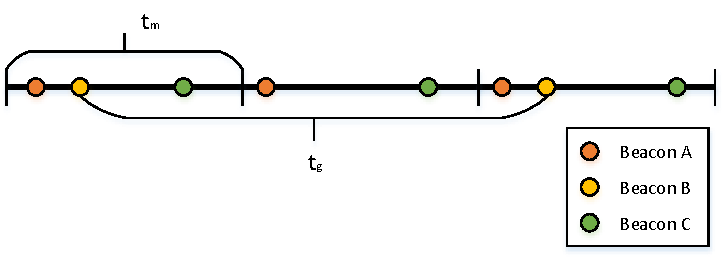
\includegraphics[width=1.0\linewidth]{Bilder/Lok-Messung}
\caption{Pseudogleichzeitigkeit bei Messungen}
\label{fig:Lok-Messung}
\end{figure}

Abbildung \ref{fig:Lok-Messung} zeigt ein Zeitintervall für drei Messungen. Die
Punkte auf dem Zeitstrahl deuten eine Einzelmessung für ein bestimmtes Beacon
an.
Man sieht, dass in der zweiten Messung kein Signal für Beacon B empfangen wurde.
Da jedoch die letzte Messung dieses Beacon weniger als $t_g$ zurückliegt, tragen
wir in der Messung den Wert aus der letzten Messung ein.
In unserem Projekt haben wir $t_g = 2 \cdot t_m$ gewählt, so dass ein nicht mehr
erreichbarer Beacon spätestens nach zwei Messintervallen als nicht vorhanden
erkannt wird.

\subsection{Machbarkeitsanalyse}

Nachdem wir unseren Messvorgang definiert haben, analysieren wir anhand
einer einfachen Raumerkennung mit zwei Räumen und zwei Beacons, ob eine
Unterscheidung der Räume anhand der Messungen möglich ist.
Dazu werden wir die Verteilung der Messwerte sowohl statistisch als
auch grafisch aufbereiten.

In dieser Analyse haben wir zwei Räume gescannt, die im Folgenden als
Küche und Flur bezeichnet werden. In jedem Raum wurde ein Beacon platziert.
Die Beacons hatten folgende Bluetooth-Adressen:
\begin{itemize}
	\item 7C:2F:80:8D:E2:3B (platziert in Küche)
	\item 7C:2F:80:8D:E2:45 (platziert in Flur)
\end{itemize}
Da sich die Adressen nur in der letzten Stelle unterscheiden, referenzieren
wir diese Beacons im Folgenden nur mit diesem Teil der Adresse, d. h.
3B und 45.

\subsubsection{Statistische Aufbereitung}

Zunächst betrachten wir den Minimal-, Maximal, Mittelwert und die Standardabweichung für jeden
Beacon in jedem Raum. Diese bestimmen wir per SQL aus der SQLite-Datenbank der Messwerte.
Da die Messwerte in der Datenbank als RSSI-Werte abgelegt und erst später normalisiert werden, sind die Werte in Tabelle \ref{tab:sql-analyze} nicht normalisiert.

\begin{table}[h]
	\caption{SQL-Analyse der ersten Messung}
	\label{tab:sql-analyze}
	\begin{tabular}{|c|c|c|c|c|c|}
		\hline \textbf{Raum} & \textbf{Tag} & \textbf{min(RSSI)} & \textbf{max(RSSI)} & \textbf{avg(RSSI)} & \textbf{stddev(RSSI)} \\
		\hline 
		\hline Küche  & 3B & -82 & -40 & -60,36 & 12,46 \\ 
		\hline Küche & 45 & -88 & -69 & -78,61 & 9,29 \\ 
		\hline Flur & 3B & -94 & -64 & -78,67 & 9,95 \\ 
		\hline Flur & 45 & -83 & -49 & -67,38 & 7,53 \\ 
		\hline 
	\end{tabular}
\end{table}


\vspace{0.4cm}
Wie erwartet, gibt es relativ große Schwankungen bei den einzelnen Messwerten.
Allerdings lässt sich an den Mittelwerten ablesen, dass die beiden Räume
prinzipiell auseinander gehalten werden können.

\subsubsection{Grafische Aufbereitung}
\label{sec:lok-grafische-aufbereitung}

Da man sich unter einer Liste von Messwerten häufig wenig vorstellen kann,
wollen wir als Nächstes die Messung in einer Grafik visualisieren.
Abbildung \ref{fig:KuecheFlur_1} zeigt die Messungen in beiden Räumen.
Da eine Messung die Einzelmessungen für beide Beacons enthält, stellt diese
einen Punkt im zweidimensionalen Raum dar. Die Signalstärke ist in diesem
Diagramm bereits normalisiert. Die Farbe der Punkte zeigt, in welchem Raum
die Messung durchgeführt wurde (blau: Flur, gelb: Küche).

Aus der Grafik lässt sich entnehmen, dass die Messungen für beide Räume
annähernd linear separierbar sind. Es gibt gerade im Übergang zwischen den beiden
Clustern allerdings ein paar Messungen, die für eine korrekte Zuordnung 
problematisch sein können. Wir schließen daraus, dass eine zuverlässige Raumerkennung mehrere Messungen erfordert.

\begin{figure}[tbh]
	\centering
	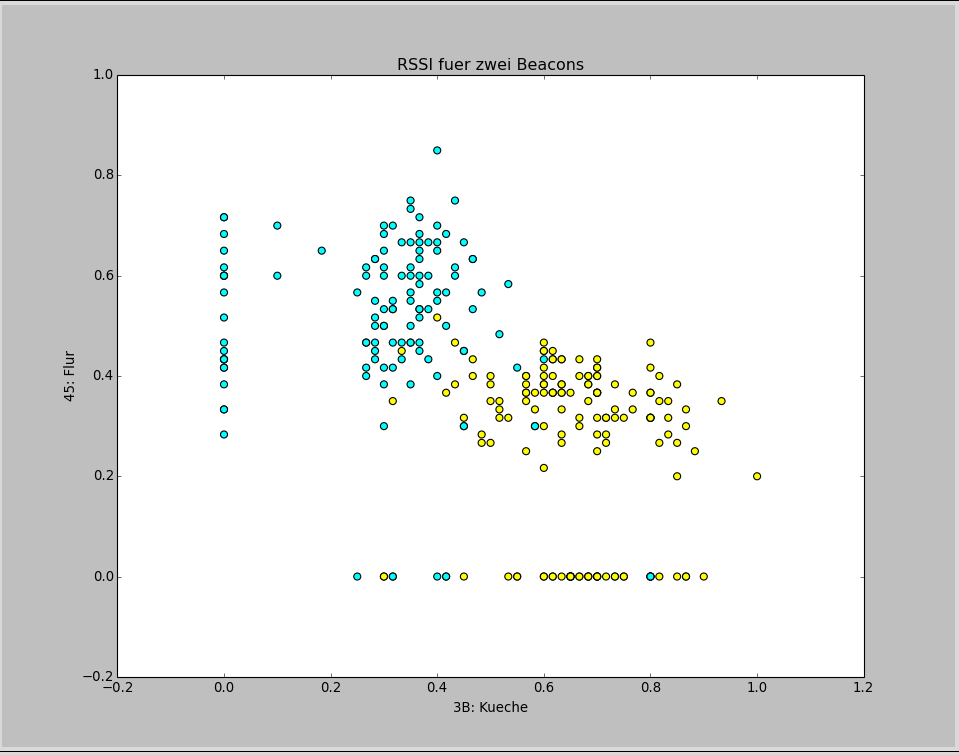
\includegraphics[width=1.0\linewidth]{Bilder/Messungen/KuecheFlur_1}
	\caption{Messung von Küche und Flur mit zwei Beacons}
	\label{fig:KuecheFlur_1}
\end{figure}

\subsection{Lösungsansatz}

Da die Machbarkeitsanalyse mit einem positiven Ergebnis abgeschlossen wurde,
entwickeln wir in diesem Abschnitt einen konkreten Lösungsansatz für die
Raumerkennung auf Basis von Messungen. Dazu erstellen wir ein Modell, dass aus
einer Reihe von Messungen den aktuellen Raum möglichst genau bestimmt.

Das Modell hat zwei Aufgaben:
\begin{enumerate}
	\item Um eine Messung einem Raum zuzuordnen, soll aus dem Messvektor der
		wahrscheinlichste Raum berechnet werden.
	\item Eine Messung allein reicht nicht aus, um eine korrekte Aussage über
		den aktuellen Raum zu machen. Deshalb sollen mehrere Messungen zu
		einer sicheren Vorhersage zusammengefasst werden.
\end{enumerate}

\subsubsection{Bestimmung des wahrscheinlichsten Raums aus einer Messung}
\label{sec:lok-wahrscheinlich}

In Abschnitt \ref{sec:lok-grafische-aufbereitung} haben wir gesehen, dass die
Messungen für unterschiedliche Räume zum großen Teil linear separierbar sind.
Allerdings gilt das nicht für die komplette Menge von Messungen.
Ein naiver Ansatz wie der Perzeptron-Algorithmus würde also nicht zum Erfolg
führen, da der Algorithmus nur konvergiert, wenn die Daten komplett linear
separierbar sind
\footnote{\url{https://www.pearsonhighered.com/assets/hip/us/hip_us_pearsonhighered/samplechapter/0131471392.pdf}}.

Daher wählen wir die etwas mächtigere Softmax-Regression, welche wir an unserer
konkreten Aufgabenstellung vorstellen wollen.
Zunächst definieren wir folgende Symbole:
\begin{itemize}
	\item Anzahl von gemessenen Beacons: $n \in \mathbb{N}$
	\item Anzahl von vermessenen Räumen: $m \in \mathbb{N}$
	\item Messung als Vektor von Einzelmessungen: $ \vec{x} \in [0, 1]^n \subset \mathbb{R}^n $
	\item Einzelmessung für Beacon $i \in [0, n - 1] \subset \mathbb{N}$: $x_i \in [0, 1] \subset \mathbb{R}$
	\item Wahrscheinlichkeitsvektor für alle Räume: $ \vec{y} \in [0, 1]^m \subset \mathbb{R}^m$
	\item Wahrscheinlichkeit für den Raum $j \in [0, m - 1] \subset \mathbb{N}$:
		$ y_j \in [0, 1] \subset \mathbb{R} $ 
\end{itemize}
\todo{Schnittmengen}

Der Messvektor $\vec{x}$ enthält die normalisierten Signalstärken für die wahrgenommenen
Bluetooth-Beacon. Er stellt die Eingabe für die Vorhersage dar. 
Der Raumvektor $\vec{y}$ besteht aus den Wahrscheinlichkeiten für die einzelnen Räume und
ist die Ausgabe der Vorhersage. Wichtig ist hier die Eigenschaft, dass sich die Wahrscheinlichkeiten
zu eins addieren:
$$ \sum_{j=0}^{m-1} y_j = 1 $$

Um aus dem Eingabevektor die gewünschte Ausgabe zu erzeugen, sind zwei Schritte notwendig.
Zuerst werden die Komponenten des Eingabevektors gewichtet summiert und mit einem Bias\footnote{Ein Bias ist ein auftretender systematischer Effekt mit einer Grundtendenz.}
versehen:

$$ z_j = \sum_{i=0}^{n-1} W_{j,i} \cdot x_i + b_j $$

Die Gleichung kann auch in Matrixform geschrieben werden:

$$ \vec{z} = W \vec{x} + \vec{b} $$

Die neu eingeführten Symbole haben folgende Bedeutung:
\begin{itemize}
	\item $W \in \mathbb{R}^{m \times n}$: Gewichtsmatrix mit $m$ Zeilen und $n$ Spalten
	\item $\vec{b} \in \mathbb{R}^m$: Bias-Vektor mit $m$ Komponenten
	\item $\vec{z} \in \mathbb{R}^m$: Nicht normalisierter Ausgabevektor mit $m$ Komponenten
\end{itemize}

Der nicht normalisierte Vektor $\vec{z}$ kann jetzt über die Softmax-Funktion normalisiert
werden\footnote{\url{http://www.gatsby.ucl.ac.uk/~chuwei/paper/smc.pdf}}:

$$ \vec{y} = \text{softmax}(\vec{z}) $$
$$ y_j = \frac{\exp(z_j)}{\sum_{k=0}^{m-1} \exp(z_k) } $$

Die Gewichtsmatrix $W$ und der Bias-Vektor $\vec{b}$ stellen Parameter der Regression dar,
die durch eine Vermessung der Räume ermittelt werden müssen. Dabei sind die Parameter so
zu wählen, dass möglichst wenig Messungen falsch eingeordnet werden. Dazu definieren wir
eine Verlustfunktion, die ein Maß für die Abweichung von der korrekten Zuordnung darstellt.
Ein Machine-Learning-Algorithmus kann diese Verlustfunktion minimieren, um
gute Parameterwerte zu bestimmen.

Wir haben als Verlustfunktion die Kreuzenthropie gewählt. Dabei werden die vom Modell vorhergesagten
Wahrscheinlichkeiten mit den korrekten Räumen aus der Vermessung kombiniert.
Sei $\vec{y'} \in \mathbb{R}^m$ der erwartete Ausgabevektor für den Raum $r$, dann gilt:
\[
y_j' = 
\begin{cases}
	1 & \text{wenn } j = r  \\ 
	0 & \text{sonst}
\end{cases}
\]
Die Verlustfunktion kann dann wie folgt definiert werden:
$$ \text{Loss}(\vec{y}, \vec{y'}) = - \sum_{j=0}^{m-1} y_j' \cdot \log(y_j) $$

Zu beachten ist, dass die so bestimmten Werte zwar alle mathematischen
Eigenschaften für Wahrscheinlichkeiten erfüllen. Allerdings können wir den Ausgabevektor
nur zur Bestimmung des Raums mit der größten Wahrscheinlichkeit nutzen,
da die konkreten Werte von der Größe der Parameter $W$ und $\vec{b}$ abhängen.

\subsubsection{Zusammenfassung von Messungen}
\label{sec:lok-zusammenfassung-messungen}

Im vorherigen Abschnitt haben wir den wahrscheinlichsten Raum für eine Messung bestimmt.
Da eine Messung keine absolut korrekte Raumerkennung leisten kann, kombinieren wir
die Ergebnisse von mehreren aufeinanderfolgenden Messungen.

Dabei betrachten wir die letzten $N$ Messungen und wählen den Raum, der in diesen
$N$ Messungen am häufigsten als wahrscheinlichster Raum bestimmt wurde.
Dies hat den Vorteil, dass einzelne Fehlmessungen nicht zu einem spontanem Raumwechsel
führen. Allerdings führt dieses Vorgehen auch eine gewisse Latenz ein, bis ein Wechsel
erkannt werden kann. Deshalb sollte $N$ weder zu klein, noch zu groß gewählt werden.
Ein weiterer Vorteil ist, dass durch diesen Ansatz ein Hysterese-Effekt entsteht.
Befindet sich der Anwender gerade im Übergang zwischen zwei Räumen, wird nicht ständig
ein Raumwechsel gemeldet, sondern erst nach einer kurzen Verzögerung.
  
\subsection{Implementierung}

Bei der Implementierung unseres Lösungsansatzes sind folgende Rahmenbedingungen zu beachten:
\begin{enumerate}
	\item Der Machine-Learning-Algorithmus zur Bestimmung der Parameter des Modells aus
		den Vermessungsdaten ist rechenintensiv und soll deshalb in einen Web-Service
		ausgelagert werden.
	\item Die Vermessung von Räumen und die Erstellung eines Modells soll nur einmalig
		erfolgen, da die Smartwatch-App offline funktionsfähig sein soll.
	\item Die Anwendung des gelernten Modells auf Messungen bei der Raumerkennung muss
		performant sein, da diese Berechnung lokal auf der Smartwatch erfolgt.
\end{enumerate}

\subsubsection{Web-Service}

Um den Machine-Learning-Algorithmus zu implementieren, haben wir uns für
TensorFlow\footnote{\url{https://www.tensorflow.org/}} entschieden.
Da diese API primär für Python entwickelt wurde, verwenden wir Python auch
für unseren Web-Service.

Der Web-Service wird als einfaches CGI-Skript in einem Apache-Server ausgeführt.
Als Eingabe werden UTF-8-kodierte Vermessungsdaten im CSV-Format erwartet.
Nachdem die Daten normalisiert und aufbereitet wurden, erstellen wir das
zuvor entwickelte Berechnungsmodell (siehe \ref{sec:lok-wahrscheinlich}) in
TensorFlow. Anschließend wird der Machine-Learning-Algorithmus auf die
Vermessungsdaten angewendet.
Das berechnete Modell wird im JSON-Format an den Client gesendet.

Das Modell enthält folgende Daten:
\begin{itemize}
	\item Gelernte Parameter: $W$, $\vec{b}$
	\item Normalisierungsinformationen: $max_{RSSI}, min_{RSSI}$
	\item Zuordnung der Beacon-Adressen und Raum-IDs zu Indizes in den Vektoren
\end{itemize}
Die Normalisierungsinformationen sind wichtig, um bei einer Messung die RSSI-Werte in
das erforderliche Intervall $[0, 1] \subset \mathbb{R}$ zu überführen.
Um beliebige Beacon-Adressen auf die korrekten Positionen im Eingabevektor $\vec{x}$
und die Komponenten im Ausgabevektor $\vec{y}$ wieder auf die betroffenen Raum-IDs
zu mappen, sind zusätzliche Zuordnungsinformationen im Modell enthalten.

\subsubsection{Offline-Fähigkeit}

Die Berechnung des Modells erfolgt im besten Fall einmalig nach Vermessen aller Räume.
Das so erstellte Modell soll auch ohne Verbindung zum Smartphone oder Internet von
der Smartwatch angewendet werden. Deshalb speichern wir das Modell als serialisiertes
Java-Objekt in den Einstellungen der Smartwatch-App über die
Preferences-API\footnote{\url{https://developer.android.com/reference/android/preference/Preference.html}}.
Da die Daten nicht relational sind, haben wir uns gegen das Ablegen in der Datenbank
entschieden.

\subsubsection{Anwendung des Modells}

Da das Modell performant auf die eingehenden Messdaten angewendet werden soll,
implementieren wir die Vektoren und Matrizen als ein- bzw. zweidimensionale
Floating-Point-Arrays. Alle Berechnungen sind in der Klasse PredictionModel
implementiert.

Die Zusammenfassung von mehreren Messungen auf eine Raumvorhersage
(siehe \ref{sec:lok-zusammenfassung-messungen}) erfolgt durch die Implementierung
einer beschränkten Queue, wobei wir als maximale Länge $N = 10$ gewählt haben.


%\section{Implementierung}
%TODO: FIXME
%
%\section{Ergebnis}
%TODO: Screenshots machen
%
%\section{Fazit}
%TODO: Unsinn formulieren


%\appendix
%\section{Anhang}

Hier kommt der Anhang.


%\newpage
%\printbibliography

\end{document}